\documentclass[conference]{IEEEtran}

\usepackage{array}
\usepackage{graphicx} % graphics package
\usepackage{float} % figure floats
\usepackage{cite}
\usepackage{epstopdf}
\usepackage{url}  % nicely format url breaks  
\usepackage{eqnarray,amsmath}
\usepackage{amsfonts}
\usepackage{amssymb}
\usepackage{pgfplots} 
\usepackage{flushend}
\usepackage{fancyhdr}    
\usepackage{multirow}
\usepackage{xcolor}
\usepackage{pgfplots} 
\pgfplotsset{compat=1.3}
\usepackage[linesnumbered, lined, ruled]{algorithm2e}
\usepackage{cite}
\usepackage{subfig}
\usepackage{comment}

\usepackage{pifont}% http://ctan.org/pkg/pifont
\newcommand{\cmark}{\ding{51}}%
\newcommand{\xmark}{\ding{55}}%

\newcommand{\red}[1]{\textcolor{red}{#1}}
\newcommand{\blue}[1]{\textcolor{blue}{#1}}

\renewcommand{\arraystretch}{1.5} % Adjust vertical spacing


\graphicspath{{Figures/}}

\hyphenation{op-tical net-works semi-conduc-tor}

\IEEEoverridecommandlockouts
\title{Low Cost Parking Spot Occupancy Detection Using Wireless Sensing} % replace it with your project title



\author{
Enes Kalinsazlioglu\\
Department of Computer Science, Virginia Commonwealth University\\
Richmond, VA 23284, USA\\
kalinsazlioef@vcu.edu\\
}


\begin{document}
% make the title area
\maketitle

\pagestyle{plain}

 \begin{abstract}

% %Write your abstract here. 200-300 words at most.
% \textit{\blue{This should include 1-2 sentence about the general context. 1-2 sentence about the problem you study and current approaches. 1-2 sentence about why your study is needed. 2-3 sentences about what you are proposing new, and \red{what you have done in this paper. 1-2 sentences about your evaluation and results, what they show. Red part is in final paper only.}  }}
% \end{abstract}

%Write your abstract here. 200-300 words at most.
\textit{This paper presents a novel, low-cost approach to accurately detecting empty parking slots using wireless sensing techniques and channel state information (CSI) data. Existing solutions either rely on dedicated sensors for each parking spot, which increases deployment costs, or estimate the total number of available spaces without pinpointing their exact locations. In contrast, our approach leverages CSI-based wireless sensing to achieve accurate, real-time detection of individual empty parking slots while maintaining cost efficiency. By utilizing CSI data, our method enables robust and reliable parking slot detection even in dynamic environments. This scalable and easily deployable solution aims to improve smart parking systems, optimizing urban mobility and parking efficiency.}
\end{abstract}

\begin{IEEEkeywords}
wireless sensing, channel state information, parking slot detection, smart parking, parking space accounting, smart cities
\end{IEEEkeywords}



 \section{Introduction}
% Around a page


% \textit{\blue{1 paragraph about the context and application and its importance.}}

% \textit{\blue{1 paragraph about your specific problem and significance.}}


% \textit{\blue{Add a motivating figure and refer to Fig.~\ref{fig:overview}. Discuss your problem through the scenario illustrated there etc.}}

% \textit{\blue{Discuss why it is novel and why this is not done before too etc.
% }}
% \newpage % remove this one once you have above content



% % figures can be in pdf, or eps format. It is ok to use png, jpeg figures too but others give better quality usually.
% \begin{figure}[t]
% \begin{center}\vspace{-6mm}
% 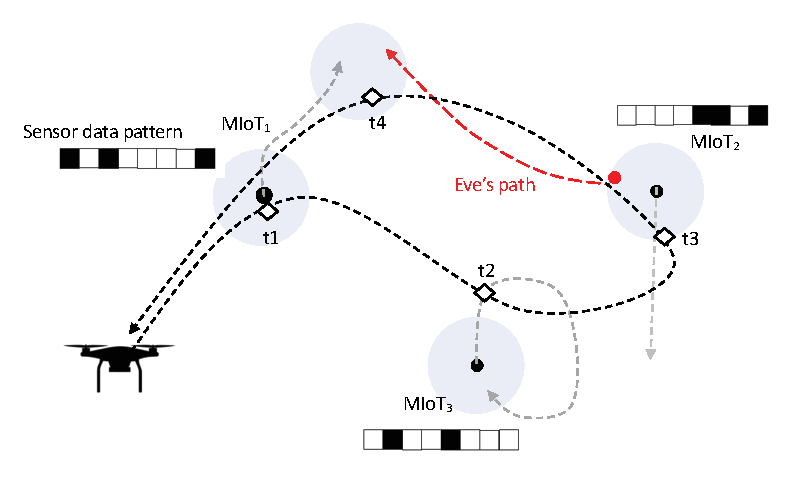
\includegraphics[width=8cm]{Figures/overview.eps}\vspace{0mm}
% \caption{\textit{\blue{Update caption and figure for your project.}} An example scenario with a UAV and three ground
% mobile IoT (MIoT) devices where the UAV needs to travel over the
% area and collect data from each IoT device securely (i.e.,
% while IoT-UAV communication is not eavesdropped) while
% optimizing the delay of the data collected.}\vspace{0mm}
% \label{fig:overview}
% \end{center}
% \end{figure}

% An example scenario is illustrated in Fig.~\ref{fig:overview}, ... 

% \textit{\blue{The last paragraph of Introduction should tell how the rest of the paper is structured. Below is just an example. Feel free to edit.}}

%  The rest of the paper is organized as follows. We discuss the related work in Section~\ref{sec:related}. In Section~\ref{sec:problem}, we provide the system model and provide the problem statement and optimization model. 
% In Section~\ref{sec:results}, we provide simulation/experimental results regarding the performance of proposed solution in various scenarios.
% Finally, we conclude and discuss future work in Section~\ref{sec:conclusion}.

% The rapid urbanization and growth in vehicle ownership have intensified the challenges associated with parking management. Efficient parking space accounting not only alleviates traffic congestion and reduces environmental impact but also improves driver satisfaction. Traditional parking management systems have evolved from manual ticketing to sophisticated sensor-based networks. Most parking decks lacks such systems due to their high cost and intrusive deployment. Recent research has leveraged wireless sensor networks (WSNs) to monitor parking space occupancy, offering a scalable and cost-effective solution for real-time parking guidance\cite{ParkingGuidanceWSN}. In parallel, various studies have demonstrated the utility of wireless sensing modalities, including Bluetooth Low Energy (BLE) and RFID, in detecting vehicle presence and managing parking operations\cite{SmartParkingMDPI, RFIDCloudArxiv}.


% Despite these advances, current approaches typically focus on either enhancing network connectivity using specific sensor technologies or employing wireless sensing for general vehicle detection rather than for precise parking space accounting. For example, BLE-based systems, while effective in communicating occupancy data, often encounter limitations in localization accuracy and robustness under varying environmental conditions\cite{SmartParkingBLE}. Similarly, studies that utilize wireless sensing for multipath analysis have primarily targeted indoor vehicle detection scenarios rather than comprehensive parking space accounting\cite{MultipathRadioSensing}. Moreover, many existing systems involve costly sensor hardware or extensive infrastructure, limiting their practical deployment in resource-constrained urban environments.


% Our research addresses these gaps by proposing a unified, low-cost framework that leverages the strengths of both wireless sensing and WSNs. By integrating these technologies, we aim to achieve higher detection accuracy, improved energy efficiency, and reduced overall system costs—attributes that are critical for large-scale implementations. This work represents a significant advancement over prior systems by unifying wireless sensing with the robust networking capabilities of WSNs, providing a holistic, low-cost approach to parking space accounting in smart city environments.





The rapid urbanization and increase in vehicle ownership have intensified challenges associated with parking management. The average American spends 17 hours per year searching for parking, resulting in an estimated \$73 billion in wasted time and fuel\cite{Inrix}. Efficient detection of empty parking slots not only alleviates traffic congestion and reduces environmental impact but also enhances driver satisfaction as well as increasing the revenue of parking facilities\cite{7895130}. Traditional parking management systems have evolved from manual ticketing to sophisticated sensor-based networks. However, many parking facilities lack such systems due to their high cost and intrusive deployment requirements.




Existing solutions for parking occupancy detection often rely on deploying dedicated sensors in each parking spot, such as magnetic or ultrasonic sensors. While these methods can provide accurate occupancy information, they significantly increase deployment and maintenance costs, making large-scale implementation economically unfeasible\cite{Polycarpou2013SmartPS}. Alternatively, some systems estimate the total number of available parking spaces without identifying the specific locations of empty slots, which limits their practicality for drivers seeking immediate parking.


Wireless sensing has emerged as a promising technology that utilizes existing wireless signals, such as Wi-Fi, to detect and interpret physical phenomena without requiring additional hardware or line-of-sight visibility. By analyzing fine-grained wireless features such as Channel State Information (CSI), wireless sensing enables applications in diverse domains. For instance, it has been used in healthcare to monitor hand movements during physical therapy exercises \cite{10.1145/3688855}, in smart buildings to perform real-time occupancy detection for energy-efficient automation \cite{10.1145/3555776.3577841}, and in activity recognition systems capable of classifying physical gestures and movements \cite{ZHURAVCHAK202259}. These studies demonstrate the versatility and robustness of wireless sensing techniques in dynamic, real-world environments. Our work builds on these principles and adapts them for the problem of detecting empty parking slots in a low-cost, non-intrusive manner.

Recent research has explored the use of wireless sensing techniques for vehicle detection as well. Most of these studies focus moving vehicles, such as those in traffic monitoring \cite{Won2017WiTrafficLA}, rather than stationary vehicles in parking lots. There are few notable studies for parking occupancy detection as well, particularly those leveraging Wi-Fi Channel State Information (CSI). For instance, WiParkFind utilizes off-the-shelf Wi-Fi devices to monitor parking occupancy by analyzing CSI data \cite{8422973}. This approach reduces the need for dedicated sensors and lowers deployment costs. However, WiParkFind focuses on estimating the number of available parking slots without pinpointing their exact locations, which can be less helpful for drivers searching for parking in real-time.

Our research addresses these gaps by proposing a low-cost, non-intrusive system that utilizes wireless sensing techniques and CSI data to accurately detect and identify individual empty parking slots. Unlike existing solutions that either require sensors for each spot or only provide aggregate occupancy counts, our approach leverages CSI-based wireless sensing to pinpoint the exact locations of vacant parking spaces. This easily accesible and deployable solution aims to improve smart parking systems, thereby optimizing urban mobility and parking efficiency.


% % figures can be in pdf, or eps format. It is ok to use png, jpeg figures too but others give better quality usually.
% \begin{figure}[t]
% \begin{center}\vspace{-6mm}
% 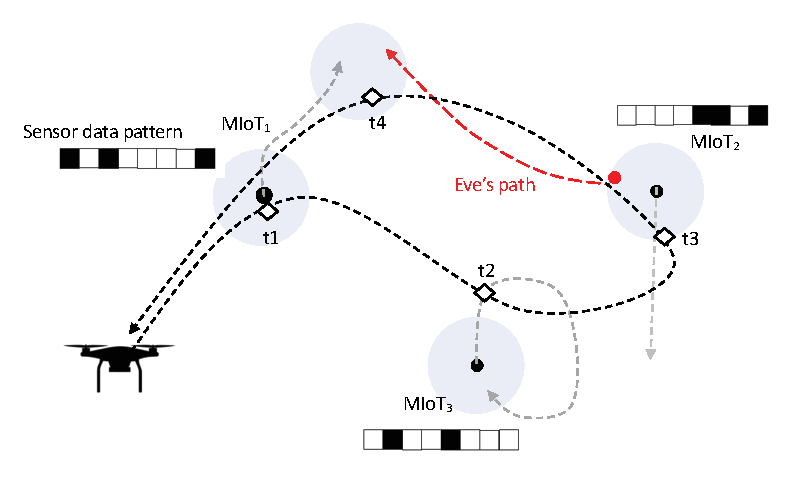
\includegraphics[width=8cm]{Figures/overview.eps}\vspace{0mm}
% \caption{\textit{\blue{Update caption and figure for your project.}} An example scenario with a UAV and three ground
% mobile IoT (MIoT) devices where the UAV needs to travel over the
% area and collect data from each IoT device securely (i.e.,
% while IoT-UAV communication is not eavesdropped) while
% optimizing the delay of the data collected.}\vspace{0mm}
% \label{fig:overview}
% \end{center}
% \end{figure}

% An example scenario is illustrated in Fig.~\ref{fig:overview}, ... 

% \textit{\blue{The last paragraph of Introduction should tell how the rest of the paper is structured. Below is just an example. Feel free to edit.}}

 The rest of the paper is organized as follows. We discuss the related work in Section~\ref{sec:related}. In Section~\ref{sec:problem}, we provide the system model and provide the steps of the proposed solution and related experiments to evaluate the performance of the proposed solution. 
In Section~\ref{sec:experimental_setup}, we provide the details of the experimental setup, including the hardware and software components used in our experiments, followed by Section~\ref{sec:experimental_results}, where we provide and describe the results of our experiments. Finally, we conclude and discuss future work in Section~\ref{sec:conclusion}.







 
\section{Related Work}
\label{sec:related}
% About 1.5-2 pages

\begin{table*}[!t]
    \begin{center}
    \caption{Comparison of proposed parking occupancy detection solutions.}
    \vspace{-1mm}
    \label{table:relatedwork}
    \begin{tabular}{| p{3.5cm}| c| c | c | c | p{6cm}|}
    \hline  
    Method/References & Coverage & Low-cost? & Non-Intrusive? & Accuracy & Other Issues and Drawbacks \\ \hline \hline
    IR Sensors\newline\cite{HumairaNishat2024IRSB, DHEEVEN2024100953} & Per-spot & \xmark & \xmark & High & Susceptible to weather and heat from sources other than vehicles \\ \hline
    Ultrasonic Sensors\newline\cite{Zhang2022ParkingDU} & Per-spot & \xmark & \xmark & High & Potential inaccuracies with soft or angled surfaces, as well as susceptibility to acoustic noise\\ \hline
    Ground Wi-Fi Sensors\newline\cite{9881350} & Per-spot & \cmark & \xmark & High & Highly impractical due to the box placed on the ground at each parking spot \\ \hline
    LoRa \& RFID Sensors\newline\cite{8938183} & Per-spot & \cmark & \xmark & High & Potential for false positives, limitations in diverse environments and challenges with robustness \\ \hline
    Vision Based\newline\cite{Agrawal2020MultiAnglePD},\cite{Bohush2019ExtractionOI},\cite{Coleiro2020CarPD},\cite{HurstTarrab2020RobustPB},\cite{Patel2020FasterRB},\cite{MartnNieto2019AutomaticVP},\cite{Pannerselvam2021AdaptivePS},\cite{Patel2020CarDB},\cite{Vtek2017ADW},\cite{Wang2023GlobalPR},\cite{Zhang2020ImageBasedAF} & Multi-spot & \cmark & \xmark & Medium & Requires high computational resources, potential privacy issues, susceptible to weather and low light  \\ \hline
    Ultra-wide-band Radar\newline\cite{Ninnemann2022MultipathAssistedRS} & Multi-spot & \xmark & \cmark & Medium & Study does not provide experimental results for cases where multiple vehicles are present  \\ \hline
    Crowd-sourcing\newline\cite{Bock2020SmartPU},\cite{7517783},\cite{10.1145/2632048.2632098} & Multi-spot & \cmark & \cmark & Low & Effectiveness heavily depends on user participation \\ \hline
    WiParkFind\cite{8422973} & Multi-spot & \cmark & \cmark & Low & Only provides vacancy count rather than pinpointing individual spots \\ \hline
    \textbf{Our work} & Multi-spot & \cmark & \cmark & High &  \\ \hline
    \end{tabular}
    \end{center}
    \vspace{-5mm}
    \end{table*}

In this section, we provide an overview of related studies in the literature. There are two main approaches for parking space accounting. While some aim to detect the presence of vehicles in individual parking spots, others focus on estimating the total number of available parking spaces. In order to achieve the former, dedicated sensors are typically deployed in each parking spot, such as magnetic or ultrasonic sensors. Studies in this area have focused on improving the accuracy of these sensors, reducing their cost, or enhancing their energy efficiency. For the latter, the method is usually based on counting the number of vehicles entering and leaving the parking lot. Since this approach is less accurate than the former, as it does not provide information about the specific locations of empty parking spaces, while being much cheaper, most of the studies in this area focus on making the individual sensor technologies more cost-effective. In order to achieve this, some studies have proposed using different sensor technologies to detect the presence of vehicles in parking spaces. Others have explored the feasibility of using fewer sensors and mitigating the need for dedicated sensors for each parking spot. For this reason, we will first review the studies that focus on individual sensor technologies for parking space accounting, and then we will review the studies that focus on using fewer sensors that can be used for multiple parking spots.

\subsection{Per-Spot Sensor Occupancy Detection}

Most of the current solutions for parking occupancy detection rely on deploying dedicated sensors in each parking spot. For example, magnetic sensors are widely used to detect the presence of vehicles in parking spaces. These sensors can be embedded in the pavement and are capable of detecting changes in the magnetic field caused by the presence of a vehicle. They are relatively inexpensive and easy to install, but they may not work well in all weather conditions or with certain types of vehicles. There are also ultrasonic sensors that use sound waves to detect the presence of vehicles. These sensors can provide accurate occupancy information, but they are more expensive and require more maintenance than magnetic sensors. 

Some studies have explored other sensor technologies for individual parking spaces. Some studies propose using infrared sensors to detect the presence of vehicles\cite{HumairaNishat2024IRSB},\cite{DHEEVEN2024100953}. These sensors can be used to detect the heat emitted by vehicles, making them suitable for outdoor environments. However, they may not work well in all weather conditions and can be affected by other heat sources in the vicinity. 

One study has proposed using a combination of different sensor technologies\cite{Zhang2022ParkingDU}. This approach combines magnetic sensors with ultrasonic sensors to improve the accuracy of parking occupancy detection and increase the battery life of the sensors.

Another approach is to use wireless signals to detect the occupancy of parking spots. For example, a study has proposed using Wi-Fi signals to detect the presence of vehicles in parking spaces\cite{9881350}. The sensor used in the study can provide accurate occupancy information and is relatively inexpensive. However, this approach requires a box to be installed on the ground of each parking spot, which can be intrusive and costly. There are studies that also focus on other wireless technologies, such as LoRa and RFID\cite{8938183}, still requiring dedicated sensors for each parking spot.


\subsection{Multi-Spot Occupancy Detection}

With the improvements in artificial intelligence and machine learning, some studies have proposed using vision-based systems for parking occupancy detection. These systems can cover multiple parking spots\cite{7895130}, process the images captured by the cameras, and detect the presence of vehicles in individual parking spaces. Most of these studies rely on deep learning algorithms to analyze the images and detect the presence of vehicles\cite{Agrawal2020MultiAnglePD},\cite{Bohush2019ExtractionOI},\cite{Coleiro2020CarPD},\cite{HurstTarrab2020RobustPB},\cite{Patel2020FasterRB},\cite{MartnNieto2019AutomaticVP},\cite{Pannerselvam2021AdaptivePS},\cite{Patel2020CarDB},\cite{Vtek2017ADW},\cite{Wang2023GlobalPR}, while others use traditional computer vision techniques\cite{Zhang2020ImageBasedAF}. In addition to the high cost and computational requirements of these systems, they also have some environmental limitations. For example, they may not work well in low-light conditions or in different weather conditions if the parking lot is not covered.

One study experimentally evaluated the performance of a ulta wide-band (UWB) radar system for parking occupancy detection\cite{Ninnemann2022MultipathAssistedRS}. The study found that the UWB radar system can accurately detect the presence of vehicles in parking spaces. However, it failed to provide results for cases where multiple vehicles are present.

There have also been studies for parking spot accounting that do not require a phsical detection of vehicles. Rather, they rely on crowd-sourced data to estimate the number of available parking spaces\cite{Bock2020SmartPU},\cite{7517783},\cite{10.1145/2632048.2632098}. These proposed solutions heavily rely on user participation and thus tend to be less accurate than the other methods. 


The closest work to our study is WiParkFind, which was briefly introduced earlier. This system uses off-the-shelf Wi-Fi devices to monitor parking occupancy by analyzing channel state information (CSI) data using machine learning\cite{8422973}. They used Intel 5300 Wi-Fi cards connected to two laptops to collect CSI data. The experiments were conducted in a parking lot with 10 spots. The researchers were able to predict the number of available parking slots with an accuracy of 78.2\%. However, WiParkFind focuses on estimating the total number of available parking slots without pinpointing their exact locations, which our study aims to address.

% \textit{\blue{You are expected to cover at least 10-15 studies that are published in the last 5-7 years.}}

% \textit{\blue{You can divide all studies covered into categories if needed and create subsections for each category.}}

% \textit{\blue{Consider creating a table to make the review of the studies easy for the reviewers. You can create columns with different features and discuss which works have that feature or component studied.
% You can also add your work in the last row and indicate that you will target all those features etc.}}






% \newpage % remove it

% % below is just example, remove it
% When UAVs are considered for data collection from ground IoT devices~\cite{wei2022uav}, 

% \textit{\blue{Talk about each paper in detail. Table~\ref{table:relatedwork} should only include key points as a summary and comparison.}}

% \newpage % remove it
% % this is used to adjust current looking without content

% \textit{\blue{Refer to Table~\ref{table:relatedwork} as you go through this section as well.}}

% \newpage % remove it

% \textit{\blue{Features in the table can be defined by your based on your application and problem. For example, if you are working on UAV networks, some features can be (i) Multiple UAVs (considered or not) (ii) Realistic mobility (iii) Energy constraint (considered or not) etc.}}








%  \section{System Model}
\label{sec:problem}

\begin{table}[t]
\begin{center}
\begin{tabular}{|p {2.6 cm} | p {5.25 cm}|}
\hline
\textbf{Notations} & \textbf{Description} \\ \hline
\hline
$\mathcal{I}$ & The set of IoT devices \\ \hline
 & \\ \hline
 & \\ \hline
 & \\ \hline
 & \\ \hline
 & \\ \hline
  & \\ \hline
 & \\ \hline
 & \\ \hline
\end{tabular}
\end{center}
\caption{Notations and their descriptions.}
\vspace{-4mm}
\label{table:notations}
\end{table}


\subsection{Assumptions}
We assume that there is a UAV and $N$ ground IoT devices, represented by set $\mathcal{I}$, ... 

\vspace{10cm}

\subsection{Problem Statement}
In the proposed scenario, the objective is to...  

\vspace{10cm}




%  \input{3-experimental_setup}
%  \vspace{-1mm}
\section{Evaluation}
\label{sec:results}


In this section, we evaluate our proposed system via simulations/experiments etc.




%  
\section{Conclusion}
\label{sec:conclusion}

% summay of your proposed solution and findings  
In this paper, we have investigated  ... problem. We proposed... We then evaluated ... The results show that...


% List how this system can be extended in the future, even if you will not be able to do it
In our future work, we plan to do....


%  \section*{Division of Work}

\textit{\blue{Discuss here, how the work is split during the preparation of this document.
In this final paper, discuss how the entire work (writing, simulations, data collection, experiments etc.) is split among project members.}}





%\newpage
\bibliographystyle{IEEEtran}

\bibliography{references}



\end{document}


